\section{Round 2: The Mixer Atlas}
\label{sec:annex-experiment-2}

This annex reports Round~2 in full. It follows the order of the published report: the parameter landscape, the training outcomes, the learning dynamics, the A$\times$B atlas, the ablation sweeps, the deployment and inference measurements, the reliability of the pipeline, and the correlations between the measured features. All numbers come from \texttt{master.csv} of the published dataset; all figures are regenerated by \texttt{make\_paper\_figures.py} from the same chart builders as the web report.

\subsection{Setup}

The population is 868 configurations: 703 hybrid-pair records (667 unique pairs after collapsing the \texttt{retnet}/\texttt{retnet\_attn} duplicate), 38 single-mixer baselines, 48 vision transformers and 79 ablations. Every run trains for 100 epochs (about 3{,}000 steps) on a 512-token Spanish vocabulary with 32-token sequences, one seed, the same warm-up-plus-cosine schedule and BitNet enabled by default. Hybrid pairs are the two-element combinations of the 42-entry mixer list, with layer~0 running mixer~A and layer~1 running mixer~B; no reversed pair exists, so the first/second asymmetry is descriptive. A pair is covered if both mixers train in every configuration that contains them: the grid has $42\times41/2 = 861$ cells and 667 were measured.

\subsection{The Parameter Landscape}

The 868 configurations span 127{,}328 to 415{,}904 parameters, with a median of 220{,}160. Hybrid pairs sit in the middle of the range because they combine two attention modules; the smallest runs are single-mixer baselines such as \texttt{attn\_single\_mamba} (127{,}328 parameters), and the largest is \texttt{engram\_\_conformer\_attn} at 415{,}904, driven by the \texttt{engram} memory bank, which adds a large key--value table to the attention block.

The composition chart is the most useful diagnostic of this section. Embeddings and the output head are fixed costs of about 49k parameters each, so any difference between configurations is paid almost entirely by the attention block and the FFN. Vision transformers are the most parameter-hungry family because they add patch embeddings and a larger classification head, while optimizer, normalization and positional-encoding ablations keep the same 210k backbone by design. Parameter cost has a clear reading: \texttt{engram} adds 100k--160k parameters wherever it appears, and \texttt{mamba} and \texttt{retnet} are among the cheapest second mixers even though they are the worst performers---cheap and bad, the worst combination.

\begin{figure}[tbp]
\centering
\fitfigure{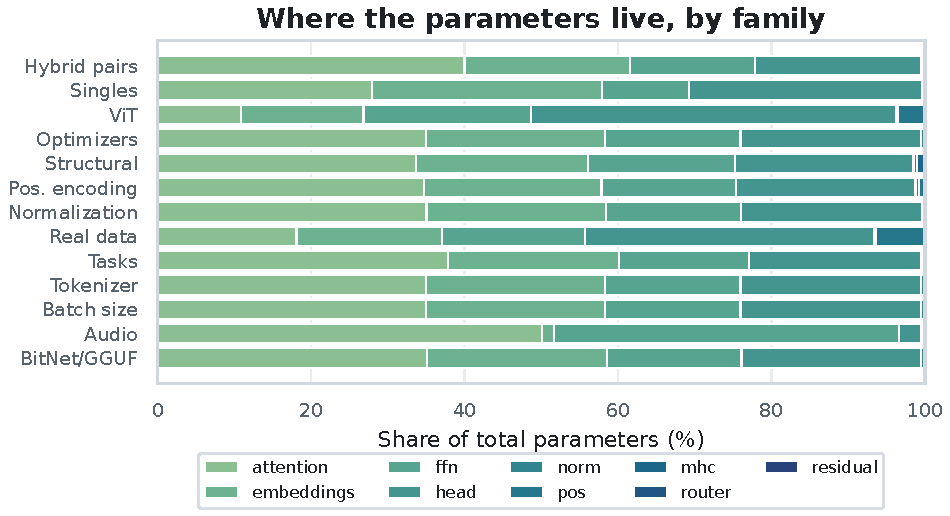
\includegraphics{figures/experiments/round2/params_composition.pdf}}
\caption{Where the parameters live, by family. Embeddings and the head are fixed costs; the attention block and the FFN carry the architectural differences.}
\label{fig:r2-params-composition}
\end{figure}

\begin{figure}[tbp]
\centering
\fitfigure{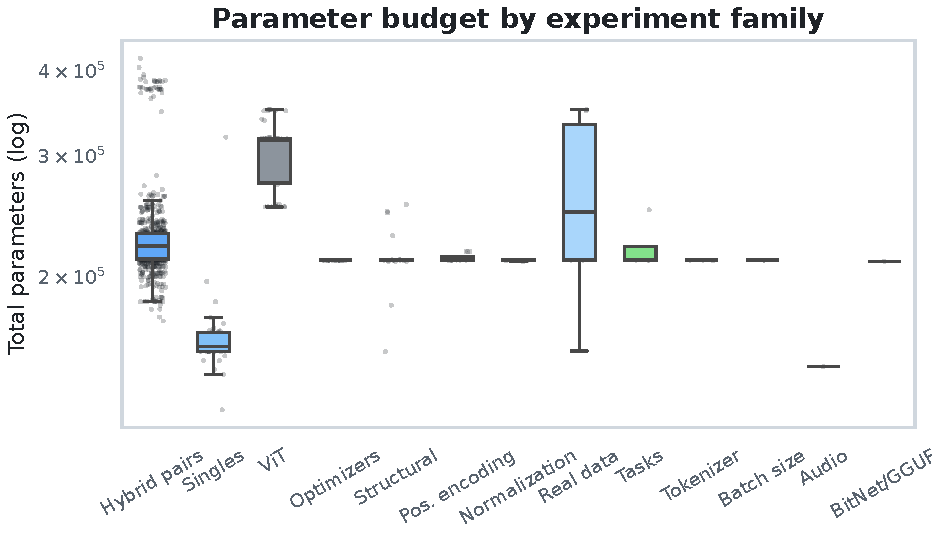
\includegraphics{figures/experiments/round2/params_family_box.pdf}}
\caption{Parameter budget by experiment family (log scale). The ViT family is the most expensive; the ablation families share one backbone.}
\label{fig:r2-params-family}
\end{figure}

\subsection{Training Outcomes}

Across the hybrid pairs, final loss ranges from 8.116 to 10.450 nats (median 9.595). The best pair is \texttt{nsa\_\_engram\_attn} at 8.116, followed by \texttt{gated\_deltanet2\_\_sparda\_attn} (8.567) and \texttt{falcon3\_\_conformer\_attn} (8.620). The worst, \texttt{gqa\_\_tucker\_attn}, needs 10.450 nats. The spread between the extremes is larger than the spread between most optimizer ablations, which is the strongest argument for choosing the attention pair deliberately.

Loss and held-out accuracy disagree. Their rank correlation over the pairs is weak, the absolute best-loss pair scores 0.0\% top-1, and the best-accuracy pair (\texttt{fox\_\_falcon1a\_attn}) reaches 12.55\% with a worse training loss (9.292). With four evaluation sentences, one lucky token rewrites the ranking, so both signals must be reported. Table~\ref{tab:r2-top-loss} lists the ten best pairs by final loss and Table~\ref{tab:r2-top-acc} the ten best by held-out accuracy.

\begin{table}[H]
\centering
\small
\caption{The ten best hybrid pairs by final training loss.}
\label{tab:r2-top-loss}
\begin{tabular}{lrrrrr}
\toprule
Pair (A + B) & Params & Final loss & Top-1 & Top-5 & Train (min) \\
\midrule
\texttt{nsa + engram}            & 383{,}999 & 8.116 & 0.00\% & 25.0\% & 154.5 \\
\texttt{gated\_deltanet2 + sparda} & 254{,}336 & 8.567 & 0.00\% & 25.0\% & 78.2 \\
\texttt{falcon3 + conformer}     & 254{,}640 & 8.620 & 4.67\% & 25.0\% & 32.6 \\
\texttt{falcon1a + conformer}    & 254{,}640 & 8.633 & 2.38\% & 25.0\% & 23.0 \\
\texttt{falcon1 + conformer}     & 254{,}640 & 8.639 & 4.67\% & 25.0\% & 21.3 \\
\texttt{fox + falcon2a}          & 222{,}768 & 8.666 & 2.40\% & 25.0\% & 84.2 \\
\texttt{gqa + conformer}         & 242{,}720 & 8.670 & 5.87\% & 25.0\% & 88.3 \\
\texttt{falcon3a + conformer}    & 254{,}640 & 8.681 & 3.97\% & 25.0\% & 23.2 \\
\texttt{fox + falcon2}           & 222{,}768 & 8.705 & 2.40\% & 25.0\% & 85.8 \\
\texttt{gla + engram}            & 387{,}296 & 8.736 & 5.17\% & 25.0\% & 149.2 \\
\bottomrule
\end{tabular}
\end{table}

\begin{table}[H]
\centering
\small
\caption{The ten best hybrid pairs by held-out top-1 accuracy.}
\label{tab:r2-top-acc}
\begin{tabular}{lrrrrr}
\toprule
Pair (A + B) & Params & Final loss & Top-1 & Top-5 & Train (min) \\
\midrule
\texttt{fox + falcon1a}         & 214{,}232 & 9.292 & 12.55\% & 0.0\% & 79.3 \\
\texttt{fox + falcon3}          & 214{,}232 & 9.618 & 12.55\% & 0.0\% & 106.1 \\
\texttt{fox + falcon3a}         & 214{,}232 & 9.235 & 12.55\% & 0.0\% & 77.3 \\
\texttt{gated\_deltanet2 + falcon2} & 250{,}216 & 9.105 & 12.41\% & 0.0\% & 80.7 \\
\texttt{gated\_deltanet2 + falcon2a} & 250{,}216 & 8.968 & 12.41\% & 0.0\% & 82.1 \\
\texttt{hgrn2 + gated\_softmax}  & 238{,}688 & 9.386 & 12.30\% & 25.0\% & 71.7 \\
\texttt{hgrn2 + tucker}          & 238{,}688 & 9.221 & 12.30\% & 25.0\% & 81.6 \\
\texttt{gqla + mlra}             & 194{,}624 & 9.461 & 11.85\% & 0.0\% & 56.0 \\
\texttt{mla + mlra}              & 194{,}624 & 9.464 & 11.85\% & 0.0\% & 86.6 \\
\texttt{deltanet + kda}          & 231{,}304 & 9.024 & 11.37\% & 0.0\% & 78.6 \\
\bottomrule
\end{tabular}
\end{table}

\begin{figure}[tbp]
\centering
\fitfigure{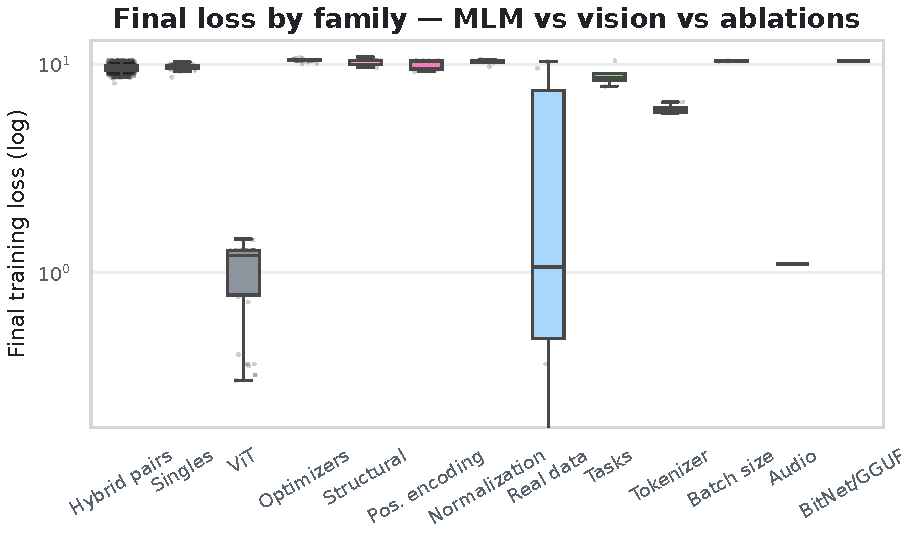
\includegraphics{figures/experiments/round2/loss_family_box.pdf}}
\caption{Final training loss by family (log scale). The vision and real-data families are not comparable with MLM losses; the families are kept separate throughout.}
\label{fig:r2-loss-family}
\end{figure}

\begin{figure}[tbp]
\centering
\fitfigure{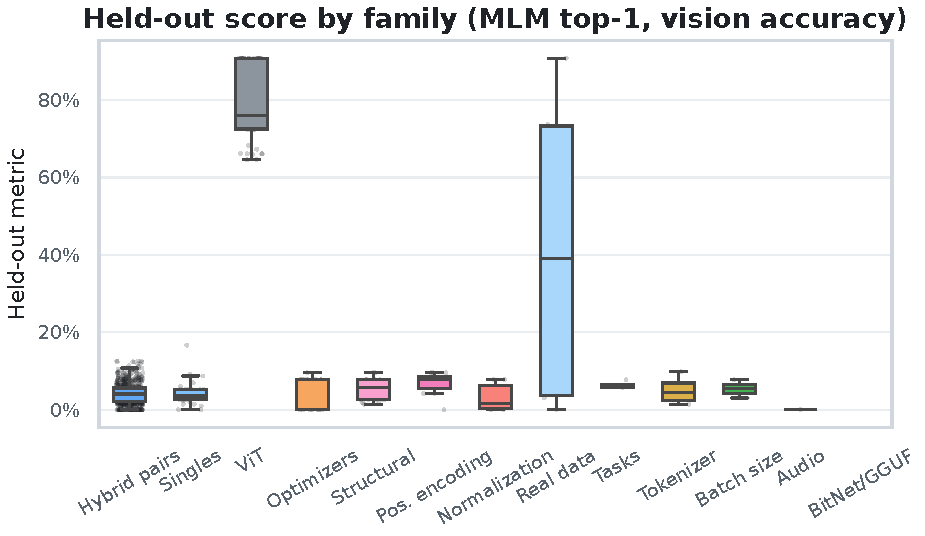
\includegraphics{figures/experiments/round2/acc_family_box.pdf}}
\caption{Held-out score by family. Vision tasks score an order of magnitude above MLM because the task is easier, not because the mixer matters more.}
\label{fig:r2-acc-family}
\end{figure}

\begin{figure}[tbp]
\centering
\fitfigure{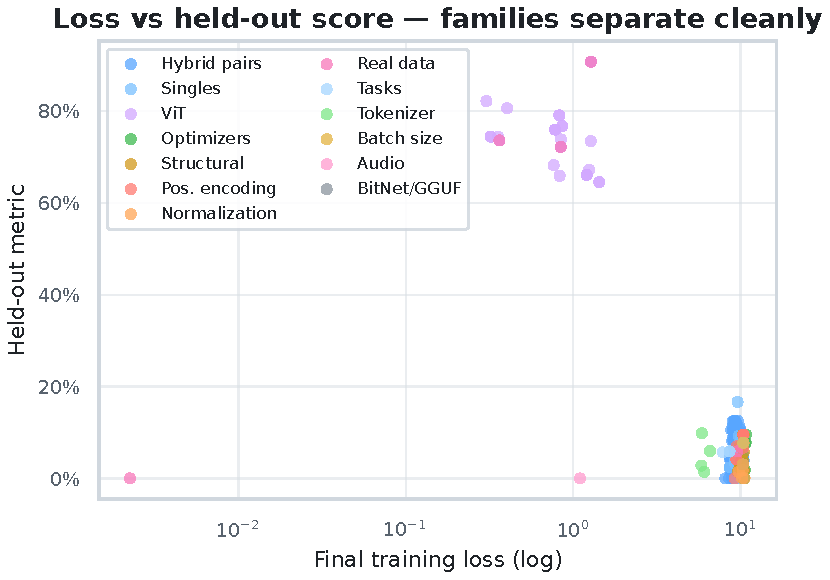
\includegraphics{figures/experiments/round2/loss_acc_scatter.pdf}}
\caption{Final loss against held-out score. The relation is weak within the pairs: the best-loss pair scores 0.0\% top-1, and the best-accuracy pair has a worse loss.}
\label{fig:r2-loss-acc}
\end{figure}

\subsection{Training Dynamics}

Every run uses the same warm-up-plus-cosine schedule, so the learning curves are directly comparable. The pair population is still descending at epoch~100: the median loss falls from about 10.2 nats at epoch~0 to 9.49 at the end. The sweep therefore measures speed of learning, not converged quality, and every ranking should be read as ``which pair learns faster in 3{,}000 steps''.

Gradient norms are stable across families (1.87 for the attention block, 0.92 for the FFN, 3.47 for the head), and the median clip ratio sits at 0.90, below the threshold of 1.0, so most steps pass unclipped and clipping only fires on spikes. The throughput median is 357 tokens/s for the pair population; the 3k--31k tail belongs to tokenizer and audio ablations whose step timer covers only part of the work, which is why the Pareto analysis excludes it.

\begin{figure}[tbp]
\centering
\fitfigure{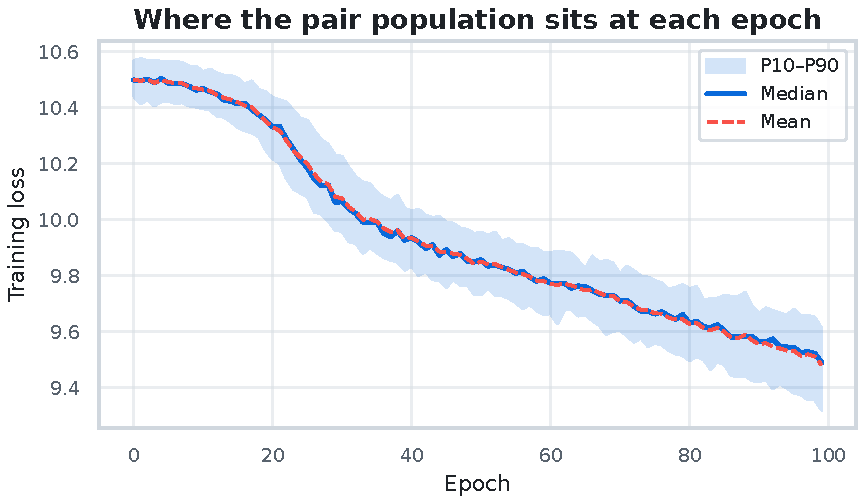
\includegraphics{figures/experiments/round2/curves_quantiles.pdf}}
\caption{Population learning curves with the P10--P90 band. The curves are still descending at epoch~100, so the sweep measures learning speed rather than converged quality.}
\label{fig:r2-curves-quantiles}
\end{figure}

\begin{figure}[tbp]
\centering
\fitfigure{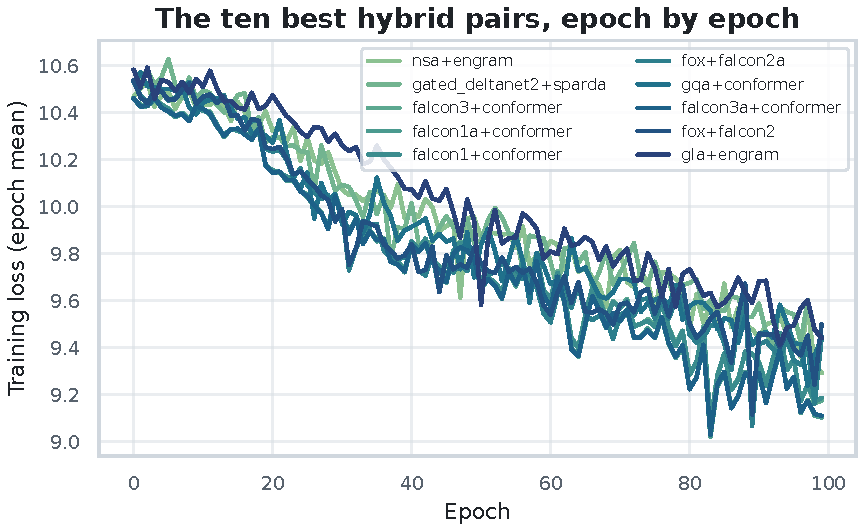
\includegraphics{figures/experiments/round2/curves_top10.pdf}}
\caption{The ten best pairs over time. The ordering is established early and rarely changes after epoch~50.}
\label{fig:r2-curves-top10}
\end{figure}

\begin{figure}[tbp]
\centering
\fitfigure{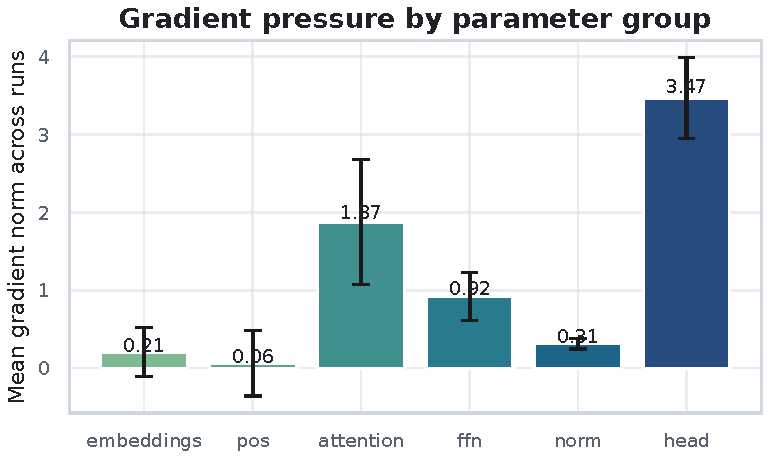
\includegraphics{figures/experiments/round2/grad_groups.pdf}}
\caption{Gradient pressure by parameter group. The head carries the largest gradient, the FFN the smallest; clipping fires rarely because the median clip ratio is 0.90.}
\label{fig:r2-grad-groups}
\end{figure}

\subsection{The A$\times$B Atlas}

The atlas is the centrepiece of the experiment: each cell is one hybrid pair, rows are the first mixer and columns the second. Read column by column, the second mixer dominates: a good B (\texttt{sparsek}, \texttt{engram}, \texttt{mlra}) keeps almost every A in the 8.9--9.6 nat band, while a bad B (\texttt{mamba}, \texttt{retnet}, \texttt{bigbird}) drags even the best A above 10 nats. Read row by row, no first mixer rescues a bad second one.

Coverage is almost complete: 667 of the 861 possible pairs were trained. The 158 pairs that never trained are exactly those containing \texttt{cca}, \texttt{ccgqa}, \texttt{msa} or \texttt{ssog}, four mixers that fail in every configuration ($4\times41 - \binom{4}{2} = 158$).

\begin{figure}[tbp]
\centering
\fitfigure{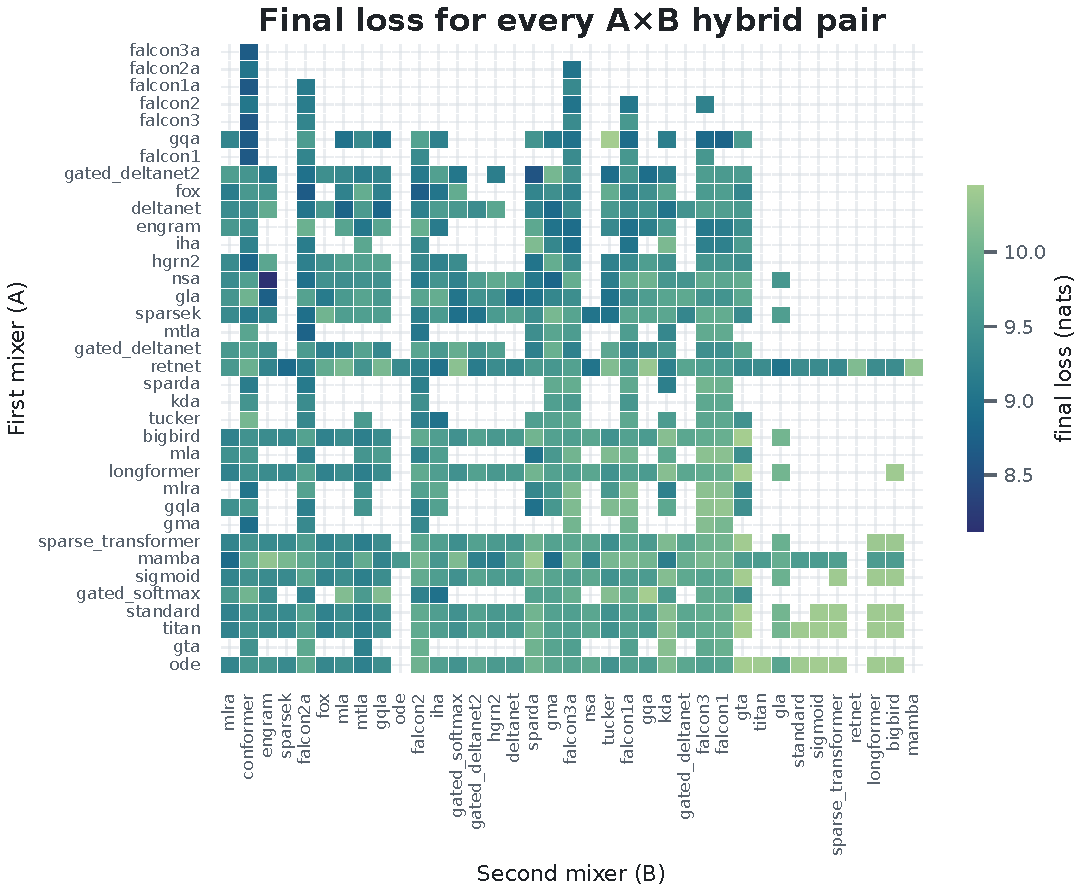
\includegraphics{figures/experiments/round2/matrix_loss.pdf}}
\caption{The A$\times$B atlas of final loss. Rows are the first mixer, columns the second; empty cells are pairs that never trained.}
\label{fig:r2-matrix-loss}
\end{figure}

\begin{figure}[tbp]
\centering
\fitfigure{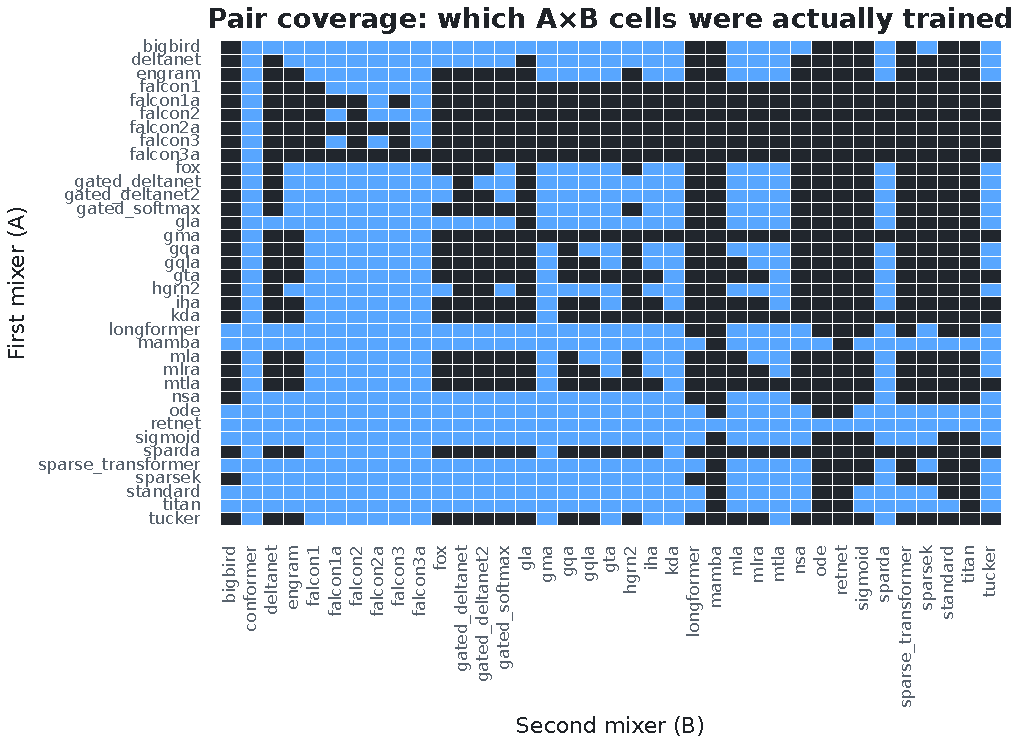
\includegraphics{figures/experiments/round2/coverage.pdf}}
\caption{Coverage of the A$\times$B grid. The missing cells are the 158 pairs that contain one of the four mixers that never train.}
\label{fig:r2-coverage}
\end{figure}

\paragraph{Which second mixer to pick.}
Table~\ref{tab:r2-best-b} ranks second mixers by mean final loss across every pair that contains them. The Pairs column shows the sample size behind each mean; a single-pair mean (for example \texttt{mamba}) is anecdotal. The bottom half is as informative as the top: \texttt{mamba}, \texttt{bigbird}, \texttt{longformer} and \texttt{retnet} are cheap but consistently drag the pair down, which is exactly the pattern the heatmaps show.

\begin{table}[H]
\centering
\small
\caption{Second mixers ranked by mean final loss over the pairs that contain them (best eight and worst eight).}
\label{tab:r2-best-b}
\begin{tabular}{lrrrr}
\toprule
Second mixer & Pairs & Mean loss & Mean top-1 & Mean params \\
\midrule
\texttt{mlra}        & 22 & 9.368 & 5.74\% & 209{,}581 \\
\texttt{conformer}   & 36 & 9.369 & 3.39\% & 259{,}861 \\
\texttt{engram}      & 18 & 9.373 & 2.05\% & 379{,}284 \\
\texttt{sparsek}     & 9  & 9.382 & 4.82\% & 208{,}926 \\
\texttt{falcon2a}    & 34 & 9.387 & 4.33\% & 229{,}973 \\
\texttt{fox}         & 16 & 9.409 & 2.23\% & 216{,}038 \\
\texttt{mla}         & 20 & 9.457 & 4.66\% & 217{,}989 \\
\texttt{mtla}        & 26 & 9.459 & 5.29\% & 217{,}223 \\
\midrule
\texttt{falcon1}     & 30 & 9.779 & 3.27\% & 221{,}856 \\
\texttt{gta}         & 25 & 9.788 & 3.27\% & 219{,}828 \\
\texttt{titan}       & 3  & 9.814 & 6.28\% & 204{,}768 \\
\texttt{gla}         & 11 & 9.814 & 3.90\% & 222{,}555 \\
\texttt{standard}    & 4  & 9.960 & 6.65\% & 206{,}264 \\
\texttt{sigmoid}     & 5  & 10.045 & 4.37\% & 207{,}162 \\
\texttt{sparse\_transformer} & 6 & 10.108 & 5.59\% & 207{,}760 \\
\texttt{mamba}       & 1  & 10.279 & 2.04\% & 192{,}608 \\
\bottomrule
\end{tabular}
\end{table}

\paragraph{Interaction beats marginals.}
The synergy chart measures how much better a pair is than the average of its two marginal means,
\[
S_{A,B} = \frac{\mu_A + \mu_B}{2} - L_{A,B},
\]
where $\mu_A$ and $\mu_B$ are the mean losses of all pairs containing A and B. \texttt{nsa+engram} gains 1.304 nats and the top ten share a pattern: a cheap, clean first mixer with a memory-heavy second one. The negative tail is dominated by \texttt{gta}, \texttt{gqa} and \texttt{tucker} as B---mixers that look average in isolation but clash when stacked after a strong A.

\begin{table}[H]
\centering
\small
\caption{The best and worst mixer interactions by synergy. Positive values mean the pair is better than its parts suggest.}
\label{tab:r2-synergy}
\begin{tabular}{lrrrr}
\toprule
Pair & Pair loss & Expected & Synergy & Top-1 \\
\midrule
\texttt{nsa + engram}          & 8.116  & 9.420 & $+1.304$ & 0.00\% \\
\texttt{gated\_deltanet2 + sparda} & 8.567 & 9.448 & $+0.881$ & 0.00\% \\
\texttt{fox + falcon2}         & 8.705  & 9.446 & $+0.741$ & 2.40\% \\
\texttt{gqa + falcon1}         & 8.784  & 9.518 & $+0.734$ & 2.86\% \\
\texttt{fox + falcon2a}        & 8.666  & 9.390 & $+0.724$ & 2.40\% \\
\midrule
\texttt{bigbird + gta}         & 10.445 & 9.725 & $-0.720$ & 1.79\% \\
\texttt{retnet + gated\_softmax} & 10.239 & 9.533 & $-0.706$ & 7.70\% \\
\texttt{mamba + engram}        & 10.277 & 9.543 & $-0.734$ & 1.10\% \\
\texttt{mamba + sparda}        & 10.391 & 9.643 & $-0.749$ & 5.09\% \\
\texttt{gqa + tucker}          & 10.450 & 9.432 & $-1.018$ & 7.76\% \\
\bottomrule
\end{tabular}
\end{table}

\begin{figure}[tbp]
\centering
\fitfigure{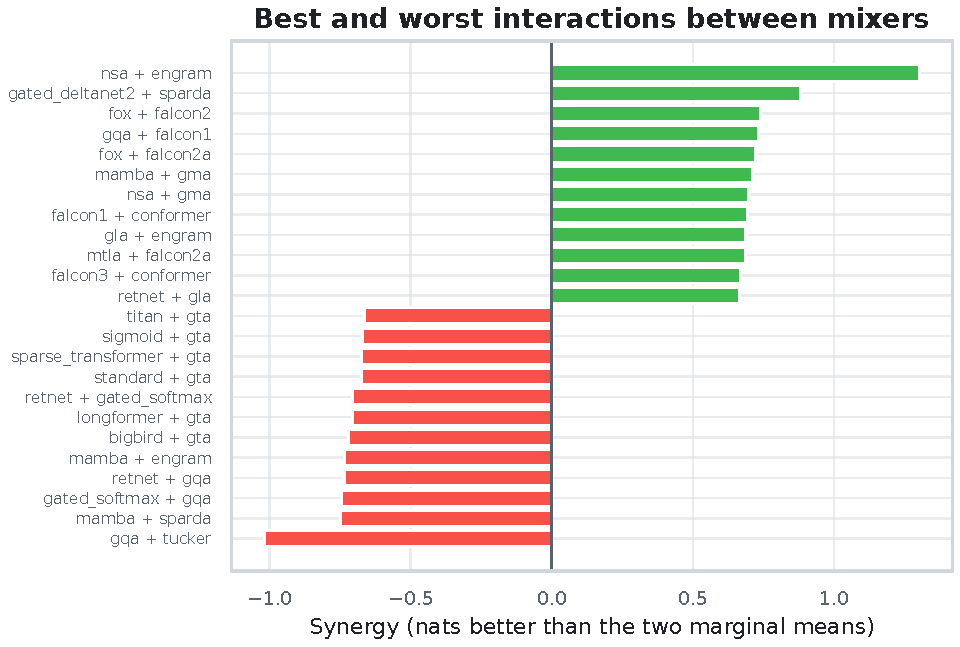
\includegraphics{figures/experiments/round2/synergy.pdf}}
\caption{Best and worst mixer interactions. The positive tail pairs a cheap, stable first mixer with a memory-heavy second one; the negative tail is dominated by second mixers that clash after a strong A.}
\label{fig:r2-synergy}
\end{figure}

\begin{figure}[tbp]
\centering
\fitfigure{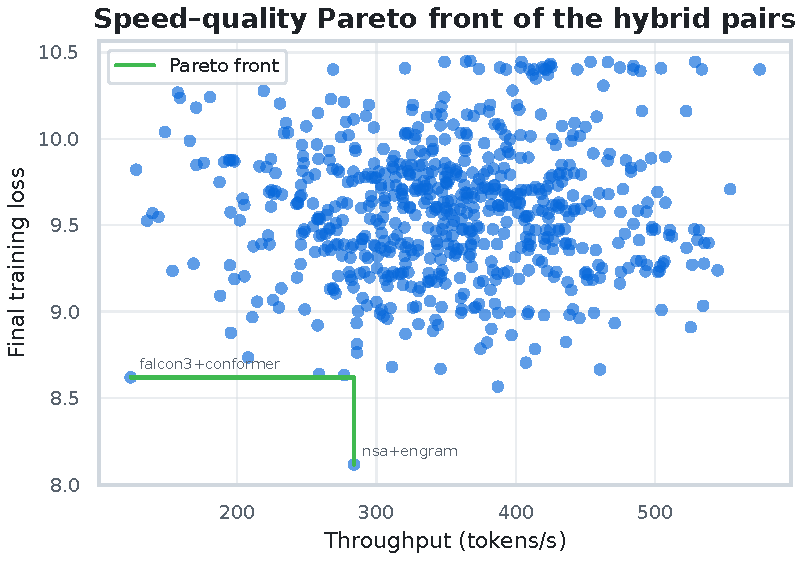
\includegraphics{figures/experiments/round2/pareto_speed_loss.pdf}}
\caption{Speed--quality Pareto front of the hybrid pairs. The front is populated by pairs whose second mixer is memory-heavy but whose first mixer is cheap.}
\label{fig:r2-pareto}
\end{figure}

\begin{figure}[tbp]
\centering
\fitfigure{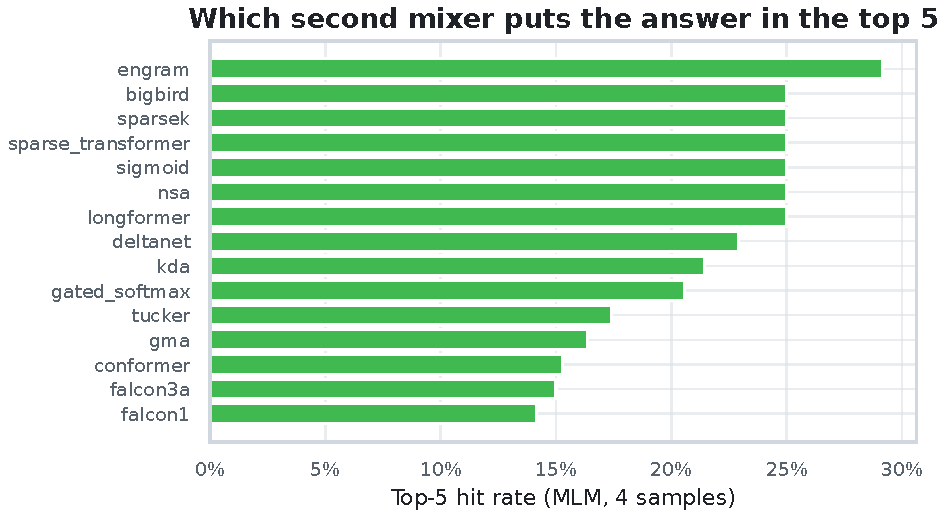
\includegraphics{figures/experiments/round2/top5_by_b.pdf}}
\caption{Top-5 hit rate by second mixer. With four samples per configuration the interval between adjacent bars is one sample, so the ordering is indicative.}
\label{fig:r2-top5-b}
\end{figure}

\begin{figure}[tbp]
\centering
\fitfigure{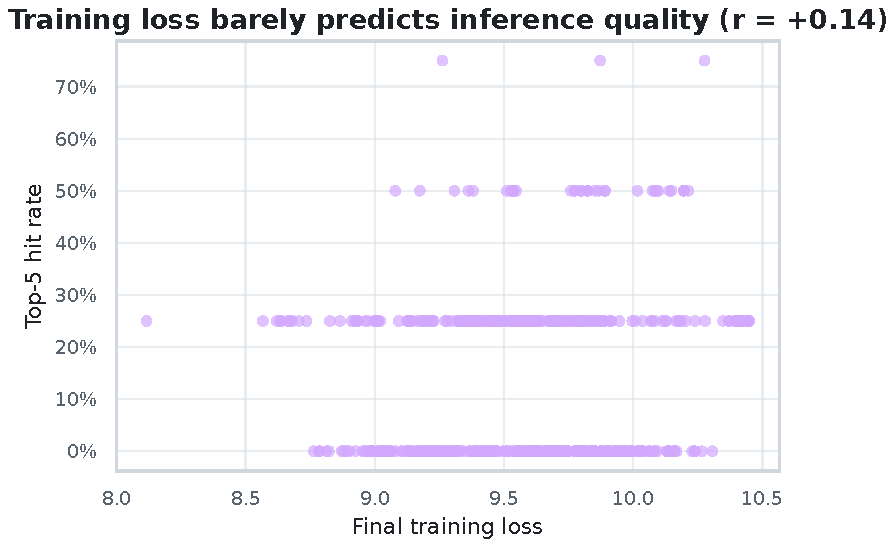
\includegraphics{figures/experiments/round2/top5_vs_loss.pdf}}
\caption{Inference quality against training loss. The correlation is weak ($r = 0.14$): training loss is not a substitute for held-out evaluation.}
\label{fig:r2-top5-loss}
\end{figure}

\subsection{Ablations}

\paragraph{Optimizers.}
The optimizer sweep is the most sobering chart: 23 optimizers, the same 210k backbone and a 10.10--10.77 nat range. \texttt{q\_apollo} wins at 10.098 and \texttt{galore\_adamw} closes the table at 10.772, but a dozen optimizers land on exactly 10.404, so the run is too short for the optimizer choice to separate from seed noise. Speed differences are real, however: step time varies by about 30\% and \texttt{shampoo} and \texttt{muon} pay visible overhead.

\begin{table}[H]
\centering
\small
\caption{Optimizer ablation: final loss, held-out top-1 and throughput on the same backbone.}
\label{tab:r2-optimizers}
\begin{tabular}{lrrr}
\toprule
Optimizer & Final loss & Top-1 & Tok/s \\
\midrule
\texttt{q\_apollo}        & 10.098 & 3.63\% & 436 \\
\texttt{sophia}           & 10.104 & 1.79\% & 378 \\
\texttt{lion}             & 10.245 & 4.64\% & 279 \\
\texttt{shampoo}          & 10.401 & 7.76\% & 382 \\
\texttt{adopt}            & 10.404 & 7.76\% & 391 \\
\texttt{mars\_adamw}      & 10.404 & 7.76\% & 343 \\
\texttt{adan}             & 10.404 & 7.76\% & 359 \\
\texttt{adamw}            & 10.404 & 7.76\% & 384 \\
\texttt{schedulefree\_adamw} & 10.404 & 7.76\% & 487 \\
\texttt{soap}             & 10.404 & 7.76\% & 412 \\
\texttt{ademamix}         & 10.404 & 7.76\% & 366 \\
\texttt{cautious\_adamw}  & 10.404 & 7.76\% & 365 \\
\texttt{prodigy}          & 10.439 & 0.00\% & 349 \\
\texttt{sgd\_momentum}    & 10.450 & 0.00\% & 347 \\
\texttt{turbo\_muon}      & 10.454 & 0.00\% & 536 \\
\texttt{anon}             & 10.458 & 0.00\% & 387 \\
\texttt{muon}             & 10.461 & 0.00\% & 507 \\
\texttt{apollo}           & 10.519 & 0.00\% & 401 \\
\texttt{adafactor}        & 10.530 & 0.00\% & 395 \\
\texttt{ada\_muon}        & 10.620 & 1.79\% & 497 \\
\texttt{lamb}             & 10.653 & 7.76\% & 464 \\
\texttt{radam}            & 10.738 & 7.76\% & 502 \\
\texttt{galore\_adamw}    & 10.772 & 9.54\% & 451 \\
\bottomrule
\end{tabular}
\end{table}

\begin{figure}[tbp]
\centering
\fitfigure{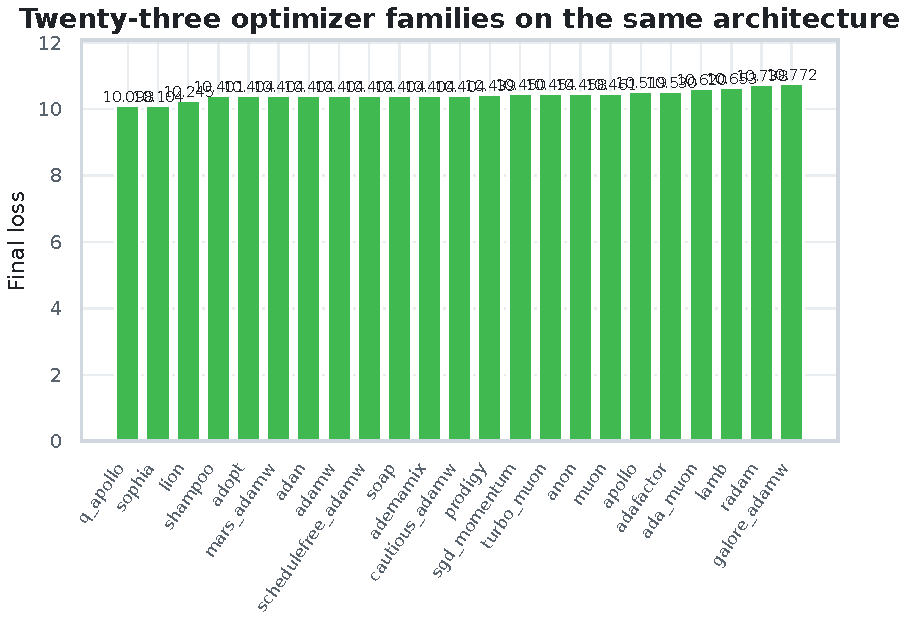
\includegraphics{figures/experiments/round2/opt_loss.pdf}}
\caption{Optimizer ablation: final loss. A dozen optimizers converge to the same value, which measures the shortness of the run more than the quality of the optimizer.}
\label{fig:r2-opt-loss}
\end{figure}

\begin{figure}[tbp]
\centering
\fitfigure{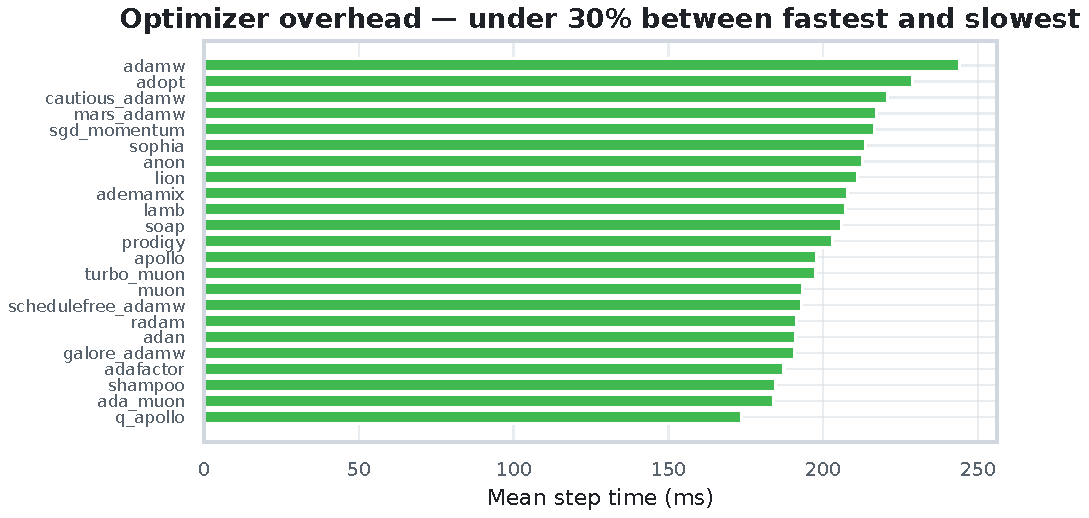
\includegraphics{figures/experiments/round2/opt_speed.pdf}}
\caption{Optimizer ablation: mean step time. The spread is about 30\%; second-order and orthogonalised methods pay the visible overhead.}
\label{fig:r2-opt-speed}
\end{figure}

\paragraph{Normalization and positional encoding.}
Among normalizations, \texttt{flash\_norm} wins clearly (9.749 nats, half a nat ahead of the runner-up), while \texttt{prms\_norm} and \texttt{rms\_norm} lag. In positional encodings the PAPE family (\texttt{pape\_ri}, \texttt{pape}, \texttt{pape\_efficient}) sweeps the podium, and classical RoPE is mid-table at this scale---a reminder that ``modern'' is not automatically better on a 100-epoch run.

\begin{table}[H]
\centering
\small
\caption{Normalization ablation on the shared backbone.}
\label{tab:r2-norms}
\begin{tabular}{lrrr}
\toprule
Variant & Final loss & Top-1 & Params \\
\midrule
\texttt{flash\_norm}    & 9.749  & 1.43\% & 209{,}600 \\
\texttt{dynamic\_tanh}  & 10.246 & 0.00\% & 210{,}752 \\
\texttt{derf}           & 10.295 & 1.79\% & 210{,}762 \\
\texttt{layer\_norm}    & 10.401 & 7.76\% & 210{,}752 \\
\texttt{rms\_norm}      & 10.436 & 7.76\% & 210{,}272 \\
\texttt{prms\_norm}     & 10.573 & 0.00\% & 210{,}272 \\
\bottomrule
\end{tabular}
\end{table}

\begin{table}[H]
\centering
\small
\caption{Positional-encoding ablation.}
\label{tab:r2-pe}
\begin{tabular}{lrrr}
\toprule
Encoding & Final loss & Top-1 & Params \\
\midrule
\texttt{pari}                 & 9.235  & 0.00\% & 211{,}520 \\
\texttt{pape}                 & 9.455  & 4.17\% & 216{,}928 \\
\texttt{pape\_efficient}      & 9.455  & 4.17\% & 216{,}928 \\
\texttt{learned\_absolute}    & 9.525  & 7.02\% & 216{,}896 \\
\texttt{hope}                 & 10.348 & ---    & 210{,}752 \\
\texttt{sinusoidal\_absolute} & 10.364 & 6.68\% & 210{,}752 \\
\texttt{bam}                  & 10.397 & 9.54\% & 210{,}768 \\
\texttt{nope}                 & 10.397 & 9.54\% & 210{,}752 \\
\texttt{none}                 & 10.397 & 9.54\% & 210{,}752 \\
\texttt{rope}                 & 10.401 & 7.76\% & 210{,}752 \\
\texttt{sinusoidal\_rotary}   & 10.401 & 7.76\% & 210{,}752 \\
\texttt{alibi}                & 10.417 & 7.76\% & 210{,}752 \\
\bottomrule
\end{tabular}
\end{table}

\begin{figure}[tbp]
\centering
\fitfigure{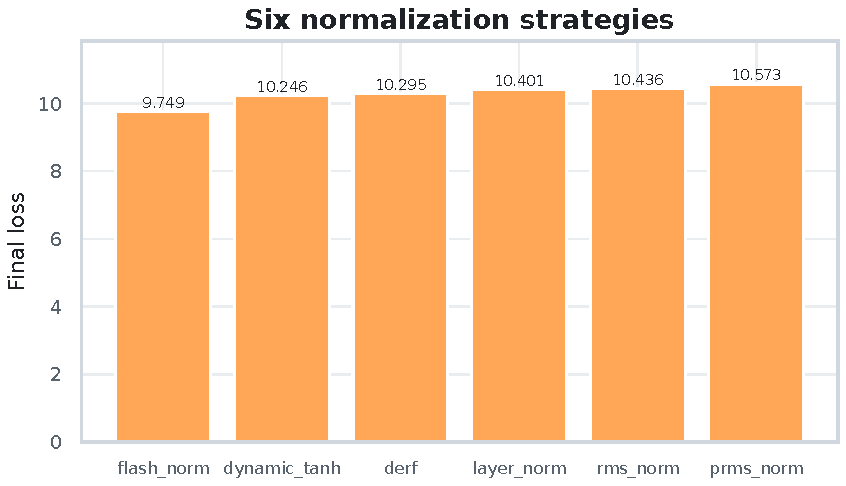
\includegraphics{figures/experiments/round2/norm_loss.pdf}}
\caption{Normalization ablation: \texttt{flash\_norm} separates from the rest by about half a nat.}
\label{fig:r2-norm}
\end{figure}

\begin{figure}[tbp]
\centering
\fitfigure{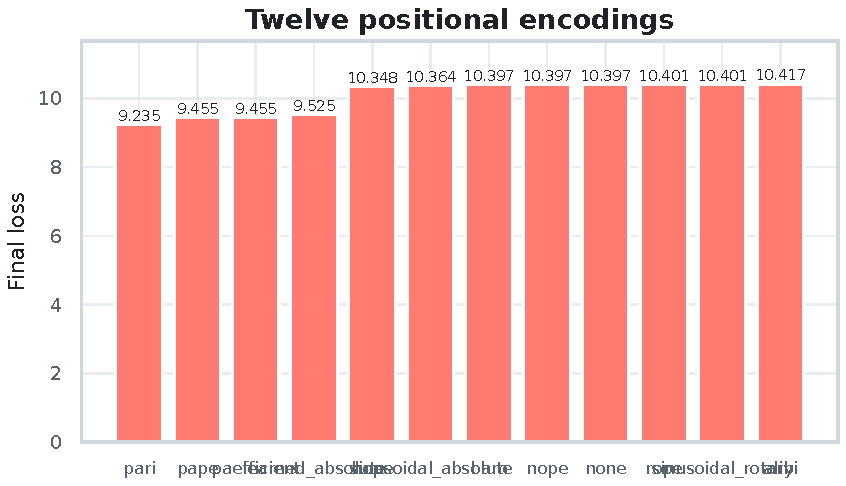
\includegraphics{figures/experiments/round2/pe_loss.pdf}}
\caption{Positional-encoding ablation: the PAPE family leads, and classical RoPE is mid-table at this scale.}
\label{fig:r2-pe}
\end{figure}

\paragraph{Structural switches.}
Structural toggles separate more than optimizers do. Factorised embeddings (9.623), SwiGLU FFN (9.901) and two Hyperloop loops (9.908) are the three wins; BitNet toggles land at 10.016, mHC at 10.186, and the residual variants at 10.43--10.49. Mixture-of-Depths is the worst switch at 10.854, consistent with its incompatibility with mHC at this depth.

\begin{table}[H]
\centering
\small
\caption{Structural switches, ordered by final loss.}
\label{tab:r2-trans}
\begin{tabular}{lrrr}
\toprule
Switch & Final loss & Top-1 & Params \\
\midrule
\texttt{factorized\_emb}          & 9.623  & 1.43\% & 181{,}056 \\
\texttt{ffn\_swiglu}              & 9.901  & 2.49\% & 228{,}800 \\
\texttt{num\_loops\_2}            & 9.908  & 6.94\% & 154{,}880 \\
\texttt{fixed\_softmax\_ssmax\_bitnet} & 9.936 & 2.60\% & 209{,}864 \\
\texttt{bitnet\_conv}             & 10.016 & 2.60\% & 209{,}856 \\
\texttt{bitnet\_on}               & 10.016 & 2.60\% & 209{,}856 \\
\texttt{mhc}                      & 10.186 & 1.79\% & 254{,}092 \\
\texttt{bitnet\_routers}          & 10.327 & ---    & 247{,}104 \\
\texttt{ssmax}                    & 10.359 & 9.54\% & 210{,}760 \\
\texttt{ffn\_relu}                & 10.393 & 3.83\% & 210{,}752 \\
\texttt{fixed\_both}              & 10.401 & 7.76\% & 210{,}752 \\
\texttt{embedding\_conv}          & 10.401 & 7.76\% & 210{,}752 \\
\texttt{fixed\_ce}                & 10.401 & 7.76\% & 210{,}752 \\
\texttt{pos\_rope}                & 10.401 & 7.76\% & 210{,}752 \\
\texttt{fixed\_softmax}           & 10.401 & 7.76\% & 210{,}752 \\
\texttt{residuals\_full\_attn}    & 10.433 & 9.54\% & 210{,}944 \\
\texttt{residuals\_none}          & 10.476 & 5.71\% & 210{,}752 \\
\texttt{moe}                      & 10.477 & ---    & 248{,}384 \\
\texttt{residuals\_block\_attn}   & 10.487 & 1.79\% & 210{,}944 \\
\texttt{mod}                      & 10.854 & --- & 210{,}944 \\
\bottomrule
\end{tabular}
\end{table}

\begin{figure}[tbp]
\centering
\fitfigure{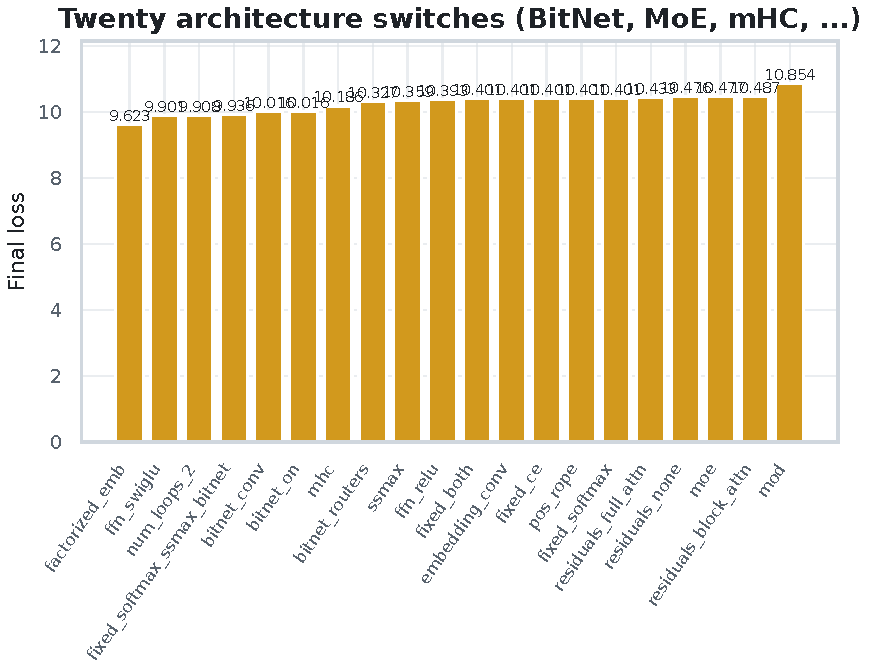
\includegraphics{figures/experiments/round2/trans_loss.pdf}}
\caption{Structural toggles. Factorised embeddings, SwiGLU and Hyperloop are the three wins; Mixture-of-Depths is the worst switch.}
\label{fig:r2-trans}
\end{figure}

\paragraph{Vision and tasks.}
The vision block works. Segmentation reaches 90.7\% mean held-out accuracy, classification 75.8\% and patch prediction 69.9\%. These scores are an order of magnitude above the MLM pairs (4.0\% median) because the task is easier, not because the mixer matters more, which is why the report keeps families separate. Tokenizer and task ablations behave as expected: the tokenizer changes the loss by several nats because it changes the vocabulary and the average sequence length, while the task changes it because the objective changes.

\begin{figure}[tbp]
\centering
\fitfigure{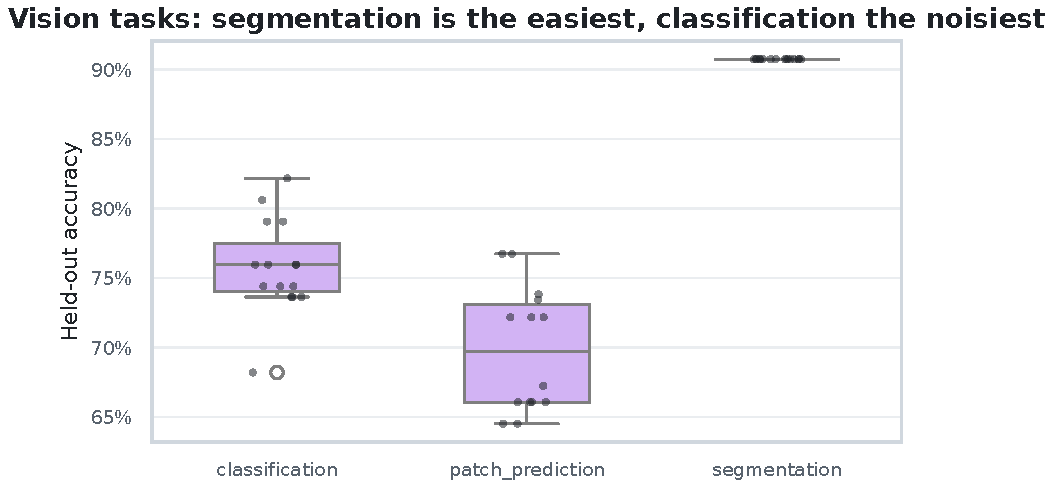
\includegraphics{figures/experiments/round2/vit_split.pdf}}
\caption{Vision tasks by objective. Segmentation is the easiest, patch prediction the hardest.}
\label{fig:r2-vit}
\end{figure}

\begin{figure}[tbp]
\centering
\fitfigure{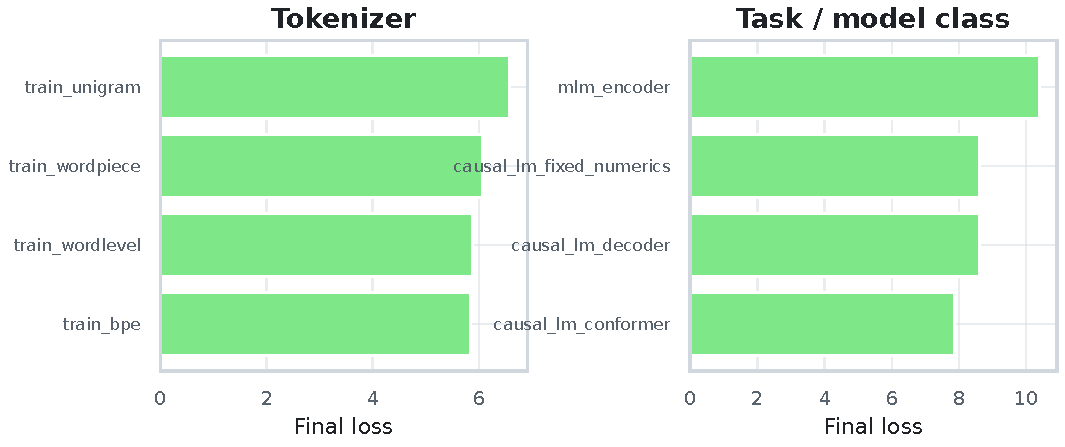
\includegraphics{figures/experiments/round2/tokenizer_task.pdf}}
\caption{Tokenizer and task ablations. Both change the loss scale, so they are not comparable with the mixer sweep.}
\label{fig:r2-tokenizer-task}
\end{figure}

\subsection{Deployment and Inference}

Post-training quantization is the good news of the round. Across the 810 configurations with both formats, mean top-1 moves from 5.62\% to 5.43\% and mean top-5 from 13.36\% to 13.24\%, deltas of $-0.19$ and $-0.12$ percentage points. Eight hundred configurations are exactly unchanged; the few that move do so by one sample out of four. For a smoke-scale model this is the expected result, but it is worth measuring rather than assuming.

The speed story is less flattering. Quantized deployment is faster than standard deployment in only 32.3\% of runs (median ratio 0.64$\times$) because the deploy stage is dominated by serialisation and conversion, not by inference; evaluation is faster 51.2\% of the time with a median 1.03$\times$ speed-up. Inference itself takes about 10.5\,s for four sentences, which is the metric that matters at serving time.

The best inference configuration is not the best-loss configuration. \texttt{mamba\_\_engram\_attn} hits three of four tokens in the top-5 (75.0\%) with a training loss of 10.277, above the pair median. With four samples per configuration, top-5 is a blunt instrument: use it to catch catastrophic failures, not to crown a winner.

\begin{figure}[tbp]
\centering
\fitfigure{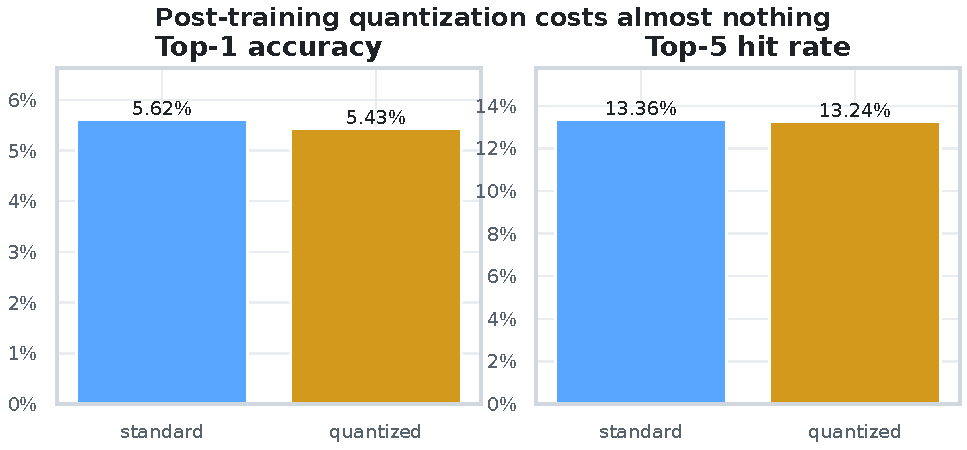
\includegraphics{figures/experiments/round2/inference_format.pdf}}
\caption{Standard versus quantized inference. The distributions overlap almost completely.}
\label{fig:r2-inference-format}
\end{figure}

\begin{figure}[tbp]
\centering
\fitfigure{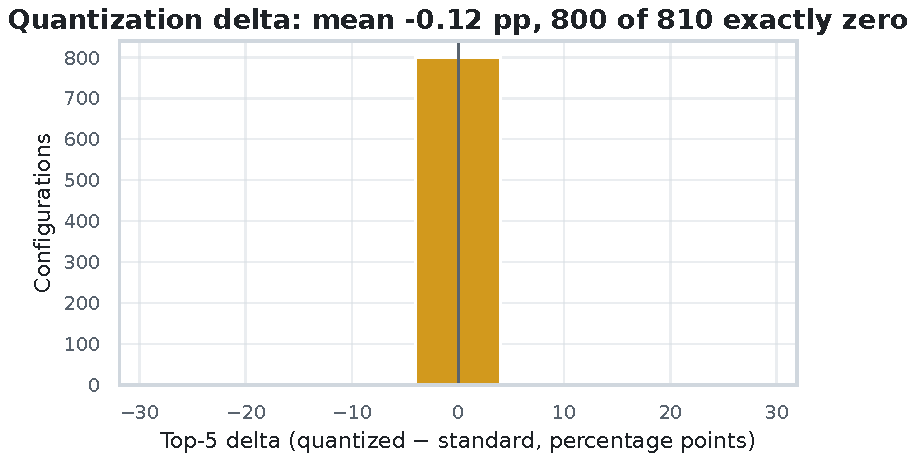
\includegraphics{figures/experiments/round2/quant_delta_dist.pdf}}
\caption{Quantization delta distribution. Eight hundred of 810 configurations have a delta of exactly zero.}
\label{fig:r2-quant-delta}
\end{figure}

\begin{figure}[tbp]
\centering
\fitfigure{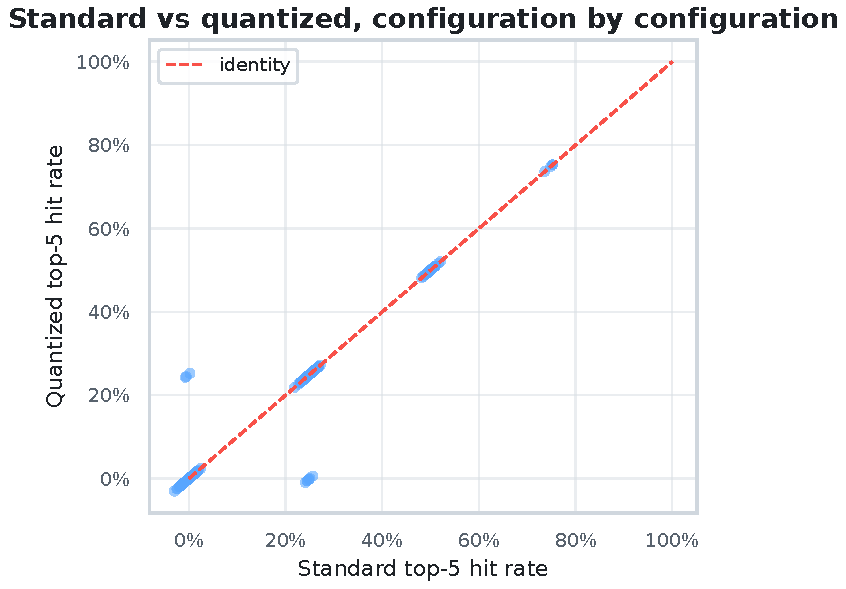
\includegraphics{figures/experiments/round2/quant_scatter.pdf}}
\caption{Standard versus quantized top-5. Every point on the diagonal is a configuration that quantization did not change.}
\label{fig:r2-quant-scatter}
\end{figure}

\begin{figure}[tbp]
\centering
\fitfigure{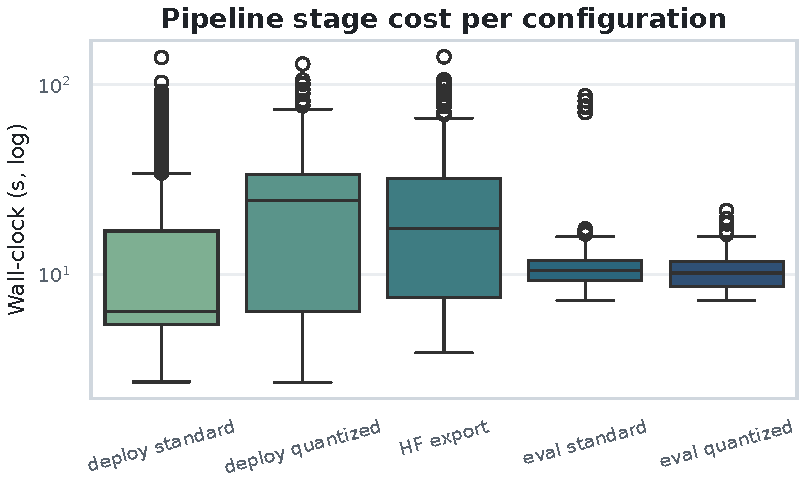
\includegraphics{figures/experiments/round2/deploy_duration.pdf}}
\caption{Pipeline stage cost. Deployment and evaluation cost seconds; training costs hours.}
\label{fig:r2-deploy-duration}
\end{figure}

\begin{table}[H]
\centering
\small
\caption{Configurations with the best standard-format top-5 hit rate.}
\label{tab:r2-inference}
\begin{tabular}{lrrrrr}
\toprule
Configuration & Top-5 std & Top-1 std & Top-5 quant & Final loss & Params \\
\midrule
\texttt{mamba\_\_engram\_attn} & 75\% & 50\% & 75\% & 10.277 & 347{,}168 \\
\texttt{mamba\_\_nsa\_attn}    & 75\% & 0\%  & 75\% & 9.262  & 192{,}479 \\
\texttt{retnet\_\_fox\_attn}  & 75\% & 0\%  & 75\% & 9.873  & 220{,}936 \\
\texttt{bigbird\_\_kda\_attn}  & 50\% & 0\%  & 50\% & 10.196 & 221{,}128 \\
\texttt{fox\_\_engram\_attn}   & 50\% & 25\% & 50\% & 9.535  & 375{,}496 \\
\texttt{fox\_\_gated\_softmax\_attn} & 50\% & 25\% & 50\% & 9.892 & 220{,}744 \\
\texttt{fox\_\_tucker\_attn}   & 50\% & 25\% & 50\% & 9.890  & 220{,}744 \\
\texttt{gated\_deltanet\_\_tucker\_attn} & 50\% & 25\% & 50\% & 9.796 & 230{,}928 \\
\texttt{gla\_\_falcon1\_attn}  & 50\% & 0\%  & 50\% & 9.511  & 226{,}032 \\
\texttt{gla\_\_mlra\_attn}     & 50\% & 25\% & 50\% & 9.538  & 211{,}808 \\
\bottomrule
\end{tabular}
\end{table}

\subsection{Reliability of the Pipeline}

The ledger records 5{,}271 stage executions. 868 training runs succeeded and 171 failed with a non-zero exit code, all of them outside the 868 analysed configurations, which were selected precisely because they trained. Deployment failed 104 times out of 1{,}734, always in symmetric pairs: a configuration that fails the standard export also fails the quantized one, which points to a shared root cause (checkpoint or configuration serialisation) rather than to quantization itself.

Two data-quality findings matter for interpretation. First, four mixers never train: \texttt{cca}, \texttt{ccgqa}, \texttt{msa} and \texttt{ssog} fail in their four singles and in all 158 pairs that contain them, which is exactly the 158 missing cells of the atlas. Second, four mixers are indistinguishable at 32-token context: \texttt{standard}, \texttt{bigbird}, \texttt{longformer} and \texttt{titan} share bit-identical losses and parameter counts because their windows (at least 64 tokens) cover the whole sequence and the position-augmented variant reduces to plain multi-head attention; they agree on all 33 shared second mixers. Separately, 37 pairs appear as \texttt{attn\_retnet\_\_X} and \texttt{attn\_retnet\_attn\_\_X} with identical metrics---two names for one implementation---which the atlas collapses to one row.

\begin{figure}[tbp]
\centering
\fitfigure{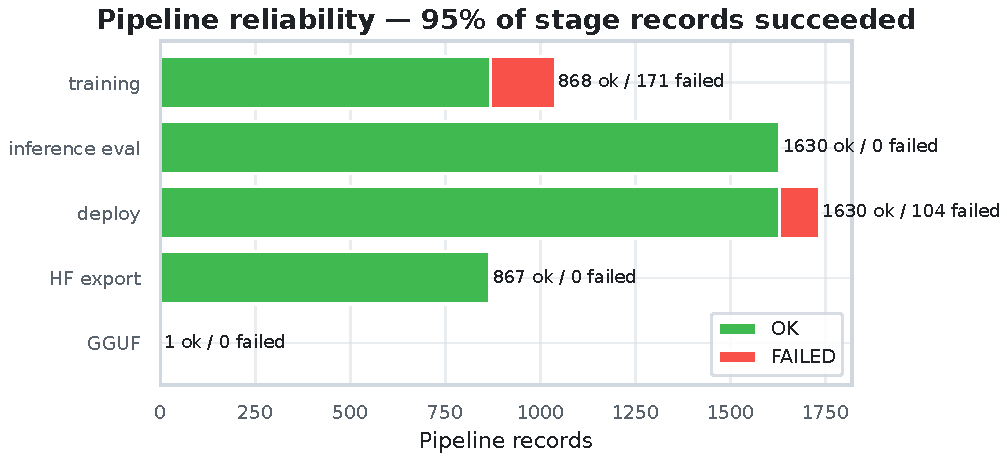
\includegraphics{figures/experiments/round2/stage_status.pdf}}
\caption{Pipeline reliability. 95\% of stage records succeeded; training and deployment account for all failures.}
\label{fig:r2-stage-status}
\end{figure}

\begin{figure}[tbp]
\centering
\fitfigure{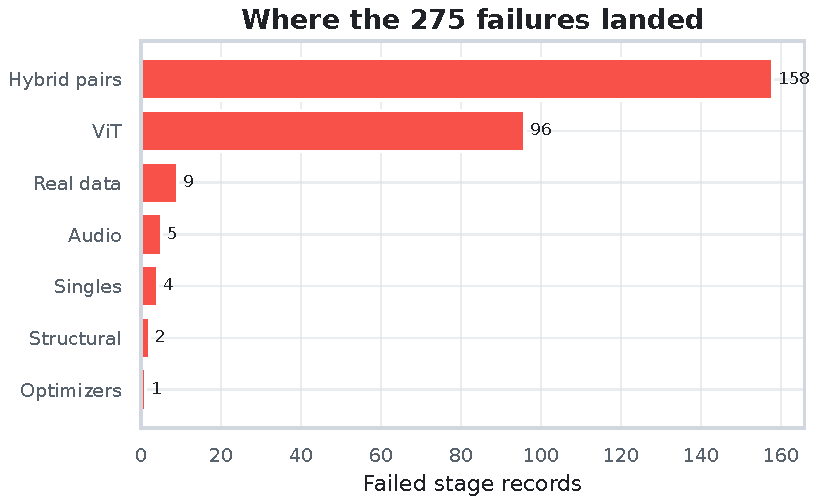
\includegraphics{figures/experiments/round2/failures_family.pdf}}
\caption{Where the 275 failures landed. Training failures cluster in the families whose mixers never train; deployment failures are symmetric across formats.}
\label{fig:r2-failures}
\end{figure}

\subsection{What Predicts Quality}

Over the hybrid pairs, parameter count correlates with final loss at $r = -0.20$ and with held-out accuracy at $r = -0.07$: size barely buys quality here. What it does predict reliably is cost ($r = 0.68$ with step time, $r = 0.65$ with wall-clock). Training loss carries only a weak signal about inference quality ($r = 0.14$ with top-5). Gradient norm and clip ratio are exactly redundant with each other ($r = 1.00$), which is expected because the clip ratio is computed from the gradient norm, and neither correlates with quality.

The correlation matrix of Figure~\ref{fig:r2-correlation} is computed over all 868 rows. Read that way, parameter count correlates with loss at $-0.43$ and with accuracy at $+0.42$, which contradicts the pair-only numbers. Both are correct: the all-rows matrix is dominated by the contrast between vision transformers (larger, much lower loss, much higher accuracy) and MLM pairs, so it measures the family gap, not the effect of size. Within the population that matters for the atlas---the hybrid pairs---size is close to irrelevant.

\begin{figure}[tbp]
\centering
\fitfigure{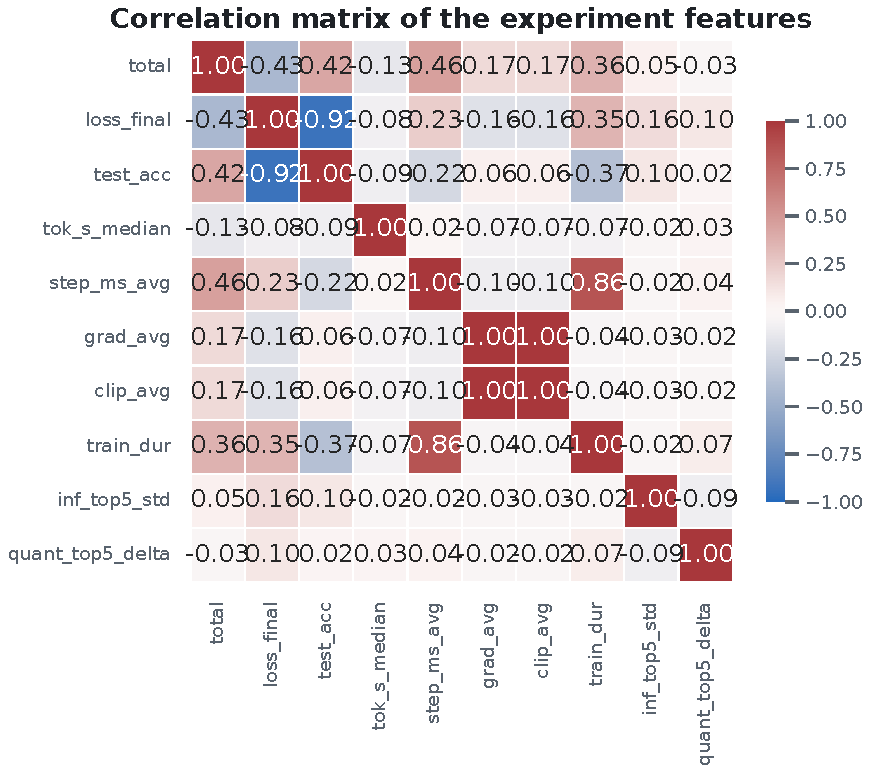
\includegraphics{figures/experiments/round2/correlation.pdf}}
\caption{Correlation matrix over all 868 configurations. The strong parameter--quality correlations are a family confound; within the hybrid pairs they fall to $-0.20$ and $-0.07$.}
\label{fig:r2-correlation}
\end{figure}

\subsection{Practical Reading and Next Steps}

If a choice must be made blind, pick a memory-heavy second mixer (\texttt{engram}, \texttt{sparsek}, \texttt{mlra}) and a cheap, stable first mixer (\texttt{fox}, \texttt{gqa}, \texttt{gated\_deltanet2}), and avoid \texttt{mamba}, \texttt{retnet} and \texttt{bigbird} as B. Expect about $\pm0.3$ nats of interaction noise, larger than the difference between most optimizers.

The round also defines its own successor. The atlas should be re-run at 256--512 tokens, where the four collapsing mixers become distinguishable and the sparse patterns actually sparsify; the evaluation should use a 200-sentence held-out set with per-token log-likelihood, because four sentences cannot rank 800 configurations; the top pairs should be trained to 300 epochs, because every curve is still descending; the \texttt{retnet} alias and the four failing mixers should be fixed or removed from the list; and at least three seeds should be run for the ablation families, where the current spread is inside seed noise. Quantization should become the default deployment format: it cost 0.12 points of top-5 and sped up evaluation in half the runs.
